\documentclass[a4paper]{article}

%% Language and font encodings
\usepackage[english]{babel}
\usepackage[utf8x]{inputenc}
\usepackage[T1]{fontenc}

%% Sets page since and margins
\usepackage[a4paper,top=3cm,bottom=2cm,left=3cm,right=3cm,marginparwidth=1.75cm]{geometry}

%% Useful packages
\usepackage{amsmath}
\usepackage{graphicx}
\usepackage[colorinlistoftodos]{todonotes}
\usepackage[colorlinks=true, allcolors=blue]{hyperref}
\usepackage{bm}


\newcommand{\vzero}{{\bf 0}}
\newcommand{\vI}{{\bf I}}
\newcommand{\vb}{{\bf b}}
\newcommand{\vd}{{\bf d}}
\newcommand{\vf}{{\bf f}}
\newcommand{\vc}{{\bf c}}
\newcommand{\vv}{{\bf v}}
\newcommand{\vz}{{\bf z}}
\newcommand{\vn}{{\bf n}}
\newcommand{\vm}{{\bf m}}
\newcommand{\vG}{{\bf G}}
\newcommand{\vQ}{{\bf Q}}
\newcommand{\vM}{{\bf M}}
\newcommand{\vW}{{\bf W}}
\newcommand{\vX}{{\bf X}}
\newcommand{\vPsi}{{\bf \Psi}}
\newcommand{\vSigma}{{\bf \Sigma}}
\newcommand{\vlambda}{{\bf \lambda}}
\newcommand{\vpi}{{\bm \pi}}
\newcommand{\valpha}{{\bm{\alpha}}}
\newcommand{\vLambda}{{\bf \Lambda}}
\newcommand{\vA}{{\bf A}}


\title{Mutect2 Strand Artifact Filter}
\author{Takuto Sato}

\begin{document}
\maketitle

\section{Introduction}
% TODO write intro

\section{The Probabilistic Model}
\begin{figure}
\centering
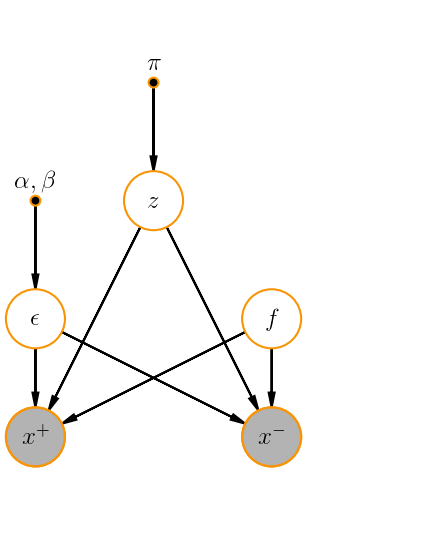
\includegraphics[width=0.3\textwidth]{strand_artifact_pgm.png}
\caption{\label{fig:frog}The probabilistic graphical model}
\end{figure}

\begin{itemize}
	\item $\vz$ is a latent random variable having a 1-of-K representation. For each variant locus, $\vz$ encodes the presence of strand artifact in forward reads ($[1, 0, 0]$), artifact in reverse reads ($[0, 1, 0]$), or no artifact ($[0, 0, 1]$)
	\item $f \sim \text{Unif}(0, 1)$ is a prior distribution over alt allele fraction $f$
	\item $\epsilon \sim \text{Beta}(\alpha, \beta)$ is a prior distribution over the error probability on a read on the artifact strand. For instance, if we have strand artifact on the reverse strand (i.e. $z = [0, 1, 0]$), $\epsilon$ is the probability that the sequencer reads a ref allele on a reverse read as alt
	\item $x^+ | f, \epsilon, z$ is the number of forward reads with the alt allele. It's a mixture of binomials, defined as follows:
	\begin{equation}
	x^+ | f, \epsilon, z \sim
		\begin{cases}
			\text{Bin} (n^+, f + \epsilon(1-f)) & z = \mathrm{Art+}\\
			 \text{Bin} (n^+, f) 			& z = \mathrm{Art-} \\
			 \text{Bin} (n^+, f)			& z = \mathrm{noArt}
		\end{cases}
	\end{equation}
\end{itemize}



We compute the conditional distributions of $x^-$  analogously.

Having observed the read counts in the forward and reverse directions, we can compute the posterior probabilities of the latent variable $z$ as described in the next section.

\section{Posterior Probabilities}

Below we derive the unnormalized posterior probability of strand artifact in forward reads ($z = art+$), given that we observed $x^+$ forward alt reads and $x^-$ reverse alt reads. We use a shorthand $z_0$ to denote $z=art+$ for conciseness. 

First we will derive the likelihood $p(x^+, x^-, f, \epsilon | z_0)$
\begin{align}
p(x^+, x^- | z_0)  &= \iint_{f, \epsilon}  p(x^+, x^-, f, \epsilon | z_0) \,df\,d\epsilon \\
			  &= \iint_{f, \epsilon}  p(f) p(\epsilon) p(x^+, x^- | z_0, f, \epsilon) \,df\,d\epsilon \\
			  &= \iint_{f, \epsilon}  p(f) p(\epsilon) p(x^+ | z_0, f, \epsilon) p(x^- | z_0, f, \epsilon) \,df\,d\epsilon \\
			  &= \iint_{f, \epsilon}  p(\epsilon) p(x^+ | z_0, f, \epsilon) p(x^- | z_0, f, \epsilon) \,df\,d\epsilon \label{watershed} \\
			  &= \iint_{f, \epsilon}  \mathrm{Beta}(\epsilon|\alpha, \beta) \mathrm{Bin}(x^+ | f + \epsilon(1-f), n^+) \mathrm{Bin}(x^- | f, n^-) \,df\,d\epsilon
\end{align}

The posterior probability of strand artifact in forward reads is therefore

\begin{align}
p(z_0 |x^+, x^-) & \propto p(z_0) p(x^+, x^- | z_0) \\
			 & = p(z_0) \iint_{f, \epsilon}  \mathrm{Beta}(\epsilon|\alpha, \beta) \mathrm{Bin}(x^+ | f + \epsilon(1-f), n^+) \mathrm{Bin}(x^- | f, n^-) \,df\,d\epsilon
\end{align}

The derivation for the probability of strand artifact on reverse strand is analogous.

For the case of no strand artifact, the derivation of likelihoods is identical up to (\ref{watershed}). Here we can simply the equation to a single integral over $f$ because the conditional probabilities of $x^+$ and $x^-$ do not depend on $\epsilon$. We use a shorthand $z_2$ for $z=\mathrm{noArt}$

\begin{align}
p(x^+, x^- | z_2)  &= \iint_{f, \epsilon}  p(\epsilon) p(x^+ | z_2, f, \epsilon) p(x^- | z_2, f, \epsilon) \,df\,d\epsilon \nonumber \\
			  &= \int_{f}  p(x^+ | z_2, f) p(x^- | z_2, f) \,df \int_{\epsilon}  p(\epsilon) d\epsilon \\
			  &= \int_{f}  \mathrm{Bin}(x^+ | f, n^+) \mathrm{Bin}(x^- | f, n^-) \,df
\end{align}

And the posterior probability is

\begin{align}
p(z_2 |x^+, x^-) & \propto p(z_2) p(x^+, x^- | z_2) \\
                         & = p(z_2) \int_{f}  \mathrm{Bin}(x^+ | f, n^+) \mathrm{Bin}(x^- | f, n^-) \,df
\end{align}

\section{Filter}
% TODO: how do we filter?

\end{document}